\chapter{Internet}
\thispagestyle{plain}

\subsection{What is internet}
Internet is a network of networks. There are hierarcical networks such as:
\begin{itemize}
    \item Internet backbone: connecting the ISPs’ backbones
    \item ISP backbone: connecting organizations’ backbones
    \item Organization backbone connects local area networks (LANs)
    \item LAN connects end systems
\end{itemize}

Internet is diveded in:
\begin{itemize}
    \item Access network: connects end systems to the first router (e.g., DSL, cable, fiber, wireless)
    \item Physical media: carries signals between devices (e.g., twisted pair, coaxial cable, fiber optic, radio waves)
    \item Network core: connects the access networks (e.g., routers and links).
    Routers work togheter to figure a path for each packet from source to destination.
    The routing table are mantained in real time and a routing algorithm can adapt to changing internet conditons.
\end{itemize}

\subsection{protocols}
Protocols specify rules about the service, such as:
\begin{itemize}
    \item procedure rules: types and sequence of messages exchanged, syntax and semantics, action to take in respect of messages and events
    \item message format size and coding
    \item timing to wait between events, timeouts, flow control
\end{itemize}

\subsection{Access layer}
Its constituted by network with end points of the same local management, provides connectivity among station on the same network and they can comunicate directly among them.

Ethernet(IEEE 802.3) is the most common access control protocol. Each host has a NIC (Network Interface Card) with a fixxed address. MAC addresses are 48bits long and uniquely identify the host in the network. Each ethernet frame has a fixed format.
\begin{figure}[H]
    \centering
    \begin{minipage}{1\textwidth}
        \centering
        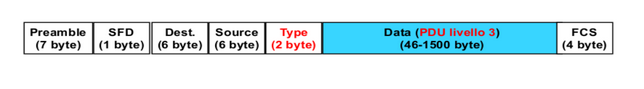
\includegraphics[width=\linewidth]{Include/Chapters/ethernet.PNG}
        \caption{Ethernet Frame Format}\label{fig:img1}
    \end{minipage}
\end{figure}

All the host connected to the same transmission system are a nework. An ethernet network costitutes a brodcast domani, where, ideally, frames sent in that domain are recived by all the host. Switches limit the explosion of the packets. Only the brodcast messages are replicated.
Switches remembers the sourca MAC address on different ports. They only replicate the frame on the segment where the MAC address replies.
Ethernet is inefficent in large network, as it uses brodcasst packets.

\section{IP}
\subsection{IP Addresses}
There are two version of IP: IPv4(32bit) and IPv6(128bit).

There are three types of IP addresses:
\begin{itemize}
    \item Unicast: identifies a single host on the network
    \item Multicast: identifies a group of hosts on the network
    \item Broadcast: identifies all hosts on the network
\end{itemize}
there are classes of IP addresses:
\begin{itemize}
    \item Class A: 24 bit for host.
    \item Class B: 16 bit for host.
    \item Class C: 8 bit for host.
    \item Class D: Used for multicast addressing.
    \item Class E: Reserved for future use.
\end{itemize}

There are routable and non routable IP addresses. The routable have to be unique on the internet, whike non routable can exist in different network but can not be used on internet.